% Chapter 4: System Design
\section{System Design}

\subsection{Overview}
This chapter documents the implemented system design of the Veritas online assessment platform. The design is grounded in the architecture and codebase described in Chapters 1--3, and it reflects the actual deployment topology, data ownership boundaries, and runtime workflows realized in the current implementation. The system follows a hybrid communication model (synchronous REST and asynchronous Kafka events), isolates data per service, and integrates AI-assisted proctoring and grading. The design decisions emphasize scalability, security, and resilience under constrained network conditions.

\subsection{Specifying the Design Goals}
The system design is guided by the objectives and constraints established in Chapter 1 and the modeling artifacts in Chapter 3. The following goals are reflected in the implemented architecture:

\begin{itemize}
    \item \textbf{Multi-tenant isolation:} Each enterprise operates within a logically isolated environment, with data stored per service and scoped by enterprise identifiers.
    \item \textbf{Hybrid communication:} Critical operations use synchronous REST calls, while domain events and consistency workflows are propagated through Kafka.
    \item \textbf{Scalability and fault tolerance:} The gateway enforces rate limits and circuit breakers, and asynchronous workflows decouple slow tasks from user-facing flows.
    \item \textbf{Integrity and auditability:} Proctoring and grading workflows generate structured evidence and enforce tamper detection in grading results.
    \item \textbf{Security-by-design:} JWT-based access control, role-based authorization, and secure token handling are applied across services.
    \item \textbf{Operational portability:} The platform runs in containerized environments including Docker Compose and Kubernetes, enabling  reproducible deployment.
\end{itemize}

\subsection{System Design}

\subsubsection{Proposed Software Architecture}
The implemented architecture follows a highly resilient microservices pattern with an API Gateway acting as the unified ingress entry point. The gateway manages security and edge operations, including token validation, tenant context resolution, rate limiting, and reverse-proxy routing to downstream internal microservices. Backend services are carefully decoupled by their bounded contexts: identity authorization (\texttt{auth-service}), corporate onboarding (\texttt{enterprise-service}), test authoring and schedules (\texttt{exam-service}), active participant environments (\texttt{candidate-service}), automated AI assessment \linebreak (\texttt{grading-service}), behavioral validation (\texttt{proctoring-service}), commercial licensing (\texttt{payment-service}), and asynchronous communications (\texttt{notification-service}). Figure \ref{fig:system-architecture} presents the architecture overview.

\begin{figure}[H]
\centering
\IfFileExists{assets/system_designs/svg_exports/system_architecture_svg-gateway.pdf}{

\includegraphics[width=1\linewidth,keepaspectratio]{assets/system_designs/svg_exports/system_architecture_svg-gateway.pdf}
}{
\fbox{\parbox{0.9\linewidth}{\centering Placeholder: System Architecture Diagram (convert SVG to PDF for final build)}}
}
\caption{System Architecture: Edge Routing and Service Interaction}
\label{fig:system-architecture}
\end{figure}

The runtime model uses synchronous HTTP for immediate operations (e.g., exam content retrieval, session validation) and Kafka for asynchronous events such as enrollment invitations, exam submissions, proctoring alerts, and subscription events. This hybrid design ensures that critical user flows remain responsive while long-running or cross-service updates remain decoupled.

Key architectural principles realized in the codebase include:

\begin{itemize}
    \item \textbf{Database-per-service ownership:} Each service owns its schema and data lifecycle. Cross-service access happens only through APIs or events.
    \item \textbf{Event-driven consistency:} Kafka topics propagate lifecycle events (enterprise suspension, exam closure, grading triggers) to keep services consistent without direct coupling.
    \item \textbf{External integration boundaries:} Third-party providers (Stripe, Cloudinary, SMTP, DeepFace, Hugging Face) are accessed only through the owning service.
\end{itemize}

\subsubsection{Subsystem Decomposition}
The system is decomposed into cohesive subsystems that map to service boundaries and operational responsibilities. Figure \ref{fig:subsystem-decomposition} shows the global decomposition, and Figure \ref{fig:subsystem-assessment} highlights assessment and session workflows.

\begin{figure}[H]
\centering
\IfFileExists{assets/system_designs/svg_exports/subsystems_decomposition_svg-global.pdf}{

\includegraphics[width=1\linewidth,keepaspectratio]{assets/system_designs/svg_exports/subsystems_decomposition_svg-global.pdf}
}{
\fbox{\parbox{0.9\linewidth}{\centering Placeholder: Subsystem Decomposition (Global) Diagram (convert SVG to PDF for final build)}}
}
\caption{Subsystem Decomposition: Global View}
\label{fig:subsystem-decomposition}
\end{figure}

\begin{figure}[H]
\centering
\IfFileExists{assets/system_designs/svg_exports/subsystems_decomposition_svg-assessment.pdf}{

\includegraphics[width=1\linewidth,keepaspectratio]{assets/system_designs/svg_exports/subsystems_decomposition_svg-assessment.pdf}
}{
\fbox{\parbox{0.9\linewidth}{\centering Placeholder: Subsystem Decomposition (Assessment) Diagram (convert SVG to PDF for final build)}}
}
\caption{Subsystem Decomposition: Assessment and Session Subsystem}
\label{fig:subsystem-assessment}
\end{figure}

\paragraph{Identity and Tenant Subsystem}
This subsystem includes Auth Service and Enterprise Service. Auth issues and refreshes JWTs, while Enterprise manages tenant onboarding, user management, and enterprise lifecycle states. Enterprise lifecycle events (suspend, delete, restore) are published to Kafka and consumed by other services to enforce cross-service consistency.

\paragraph{Assessment and Session Subsystem}
This subsystem includes Exam Service and Candidate Service. Exam Service manages question banks, exam templates, and scheduling. Candidate Service manages enrollments, session creation, answer storage, submissions, and access redemption. During submission, Candidate Service emits a slim grading trigger event, and Grading Service pulls the full payload via an internal API.

\paragraph{AI Proctoring and Grading Subsystem}
Proctoring Service handles face verification and behavioral events, aggregating cheating scores per session and publishing score updates. Grading Service consumes grading trigger events, fetches the grading payload, evaluates answers, and writes results with tamper detection and audit logging.

\paragraph{Commercial and Communication Subsystem}
Payment Service manages subscription plans, invoices, and webhooks. Notification Service consumes Kafka events and sends transactional emails for onboarding and exam events.

\subsubsection{Database Design}
The Veritas platform implements a strict \textbf{Database-per-Service} architecture to guarantee service autonomy, domain boundary enforcement, and scalable horizontal database scaling. In the current development and staging topologies, this model is implemented using logically isolated schemas within a shared PostgreSQL instance. Each service manages its own database migrations, owns its schema lifecycle, and exposes domain data exclusively through structured REST APIs or serialized Kafka messages, strictly prohibiting cross-service database joins or foreign key constraints. 

Figures \ref{fig:erd-auth} to \ref{fig:erd-proctoring} illustrate the logical Entity-Relationship Diagrams (ERD) mapping the schemas of the respective microservices.

\begin{figure}[H]
\centering
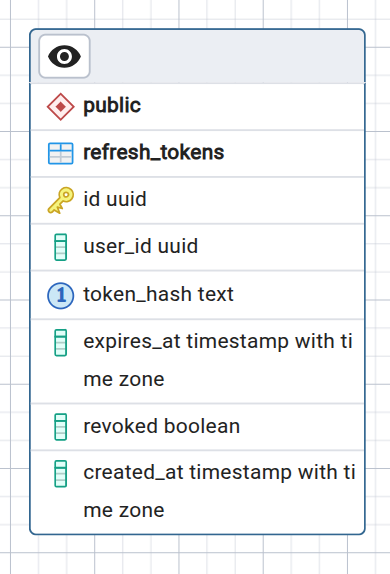
\includegraphics[width=0.95\linewidth,keepaspectratio]{assets/database_erds/auth_svc_db.png}
\caption{Auth Service Database ERD}
\label{fig:erd-auth}
\end{figure}

\begin{figure}[H]
\centering
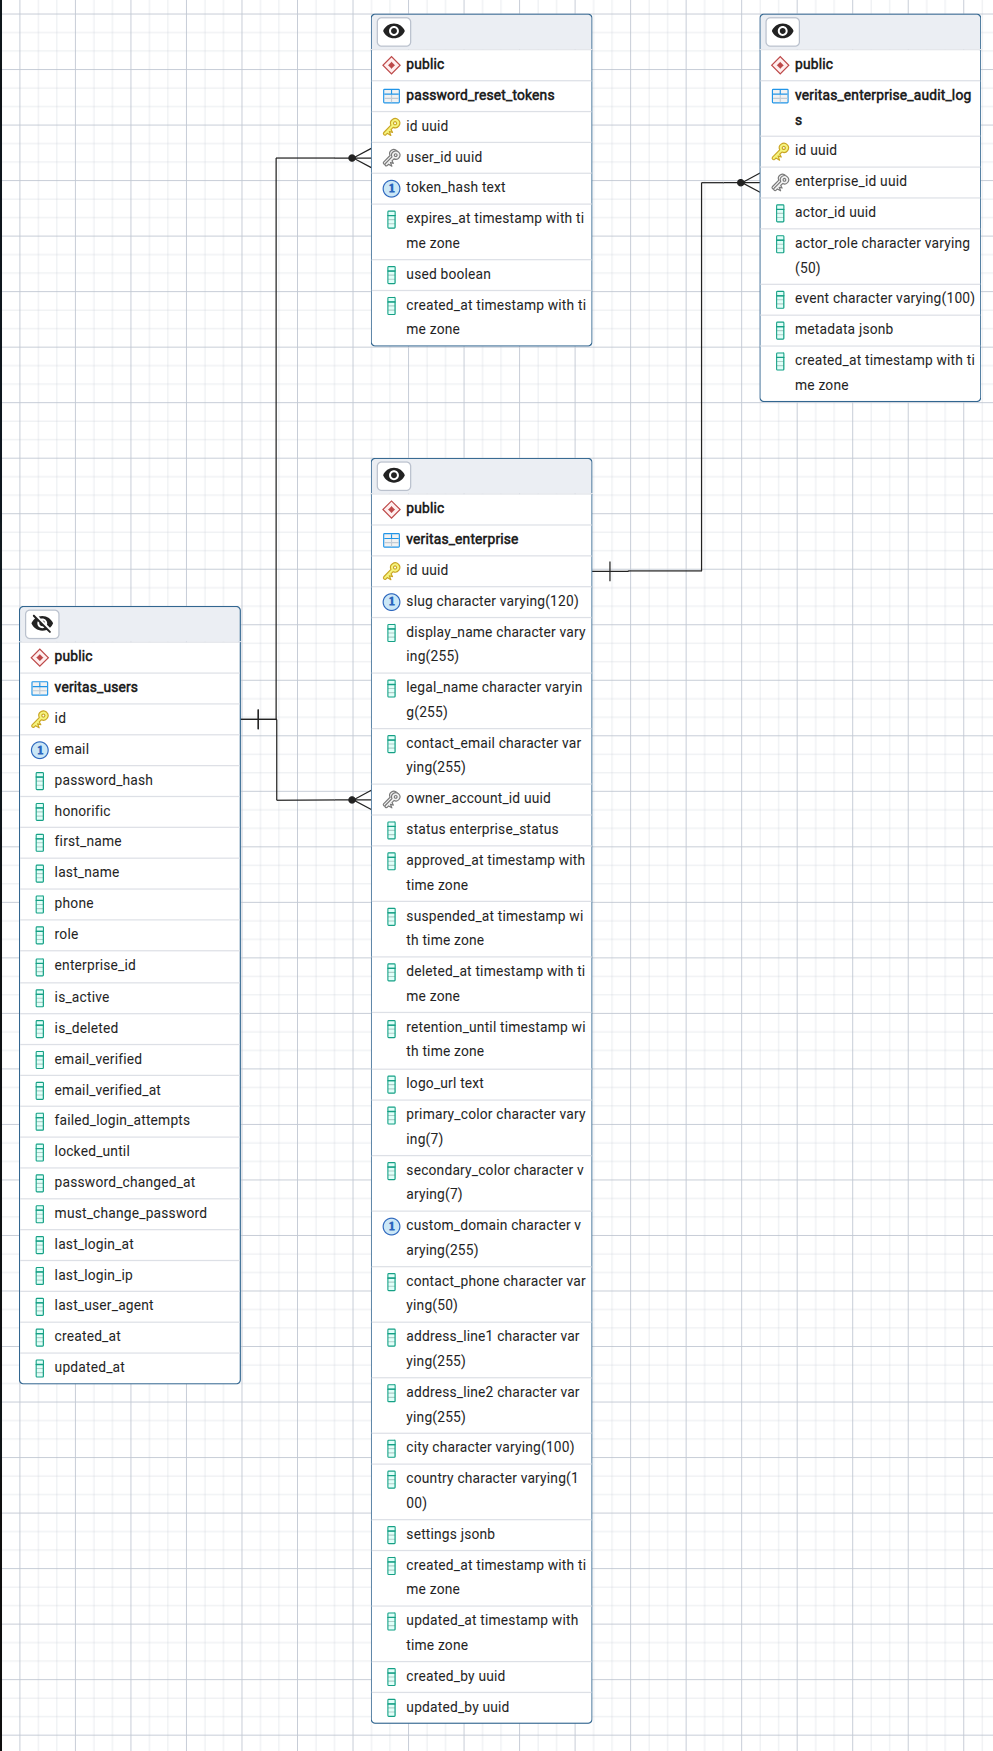
\includegraphics[width=0.95\linewidth,keepaspectratio]{assets/database_erds/enterprise_svc_db.png}
\caption{Enterprise Service Database ERD}
\label{fig:erd-enterprise}
\end{figure}

\begin{figure}[H]
\centering
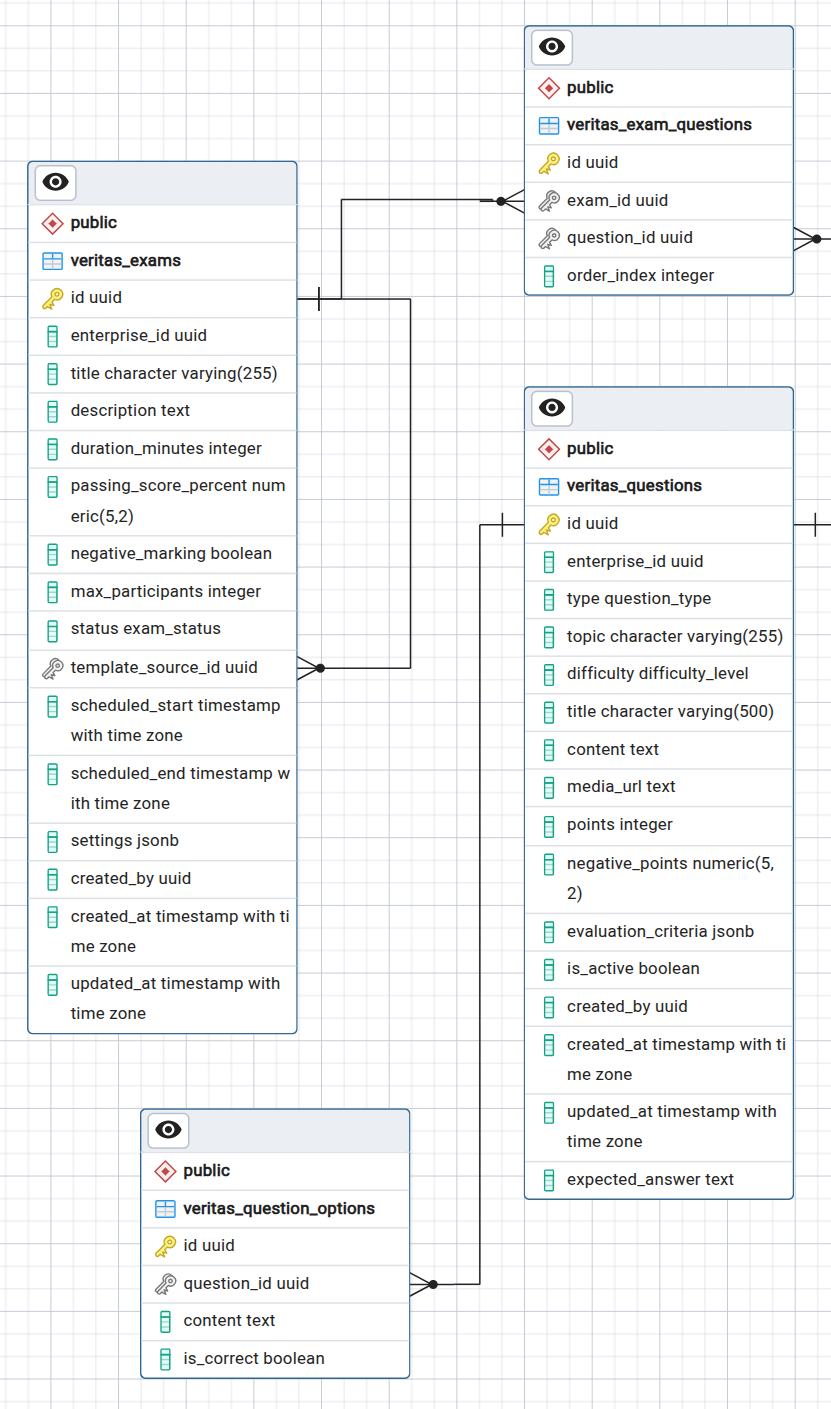
\includegraphics[width=0.95\linewidth,keepaspectratio]{assets/database_erds/exam_svc_db.png}
\caption{Exam Service Database ERD}
\label{fig:erd-exam}
\end{figure}

\begin{figure}[H]
\centering
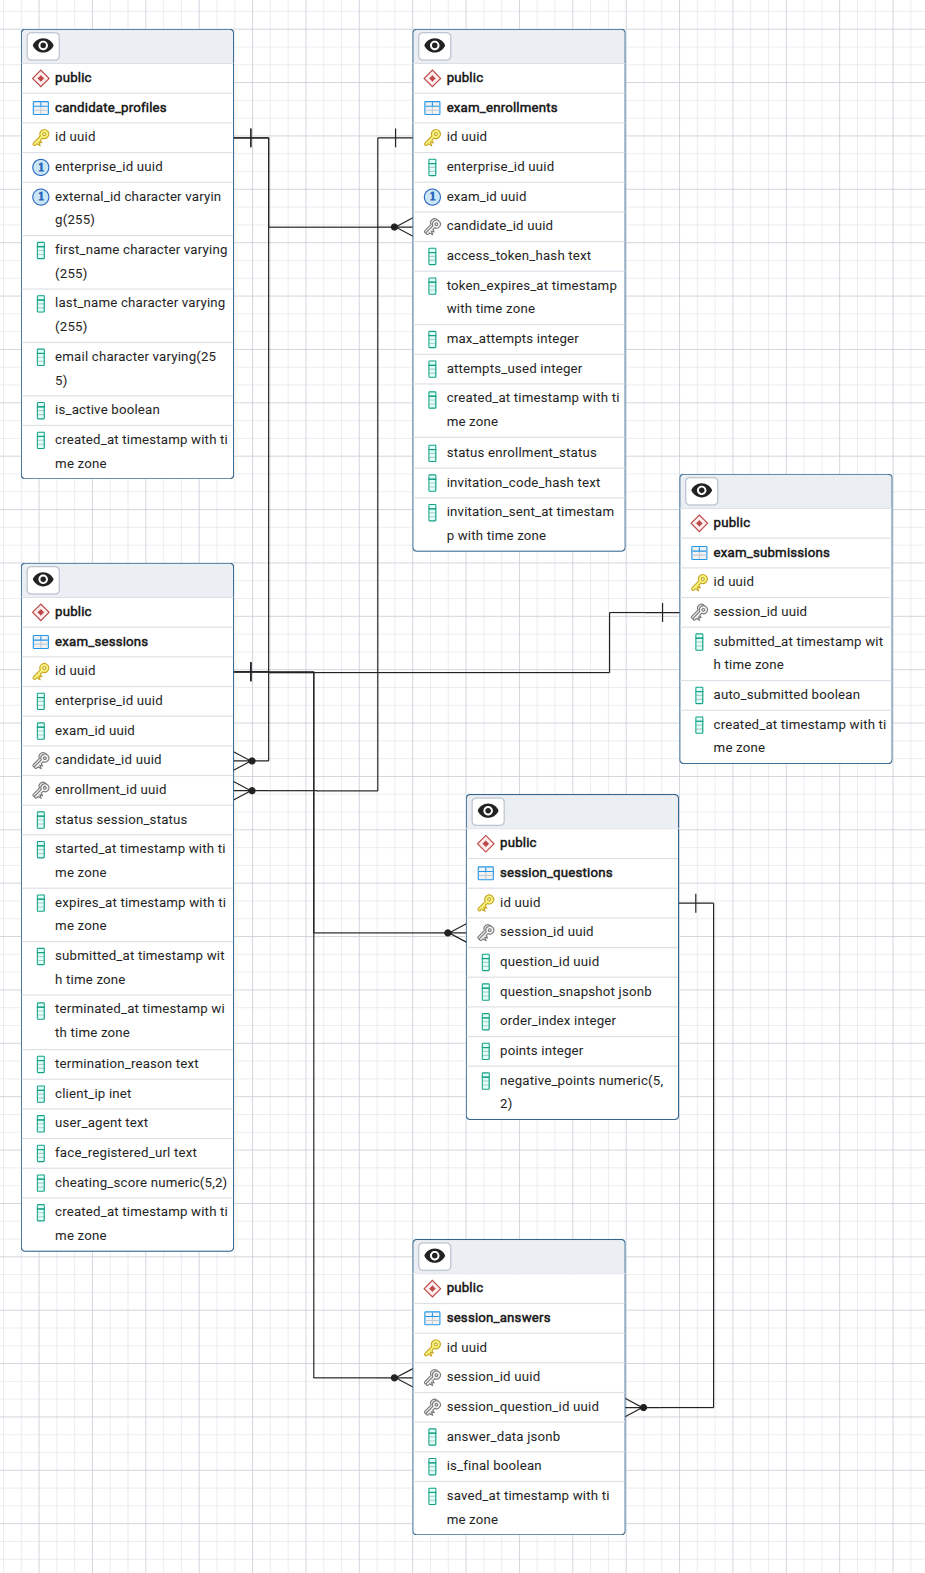
\includegraphics[width=0.95\linewidth,keepaspectratio]{assets/database_erds/candidate_svc_db.png}
\caption{Candidate Service Database ERD}
\label{fig:erd-candidate}
\end{figure}

\begin{figure}[H]
\centering
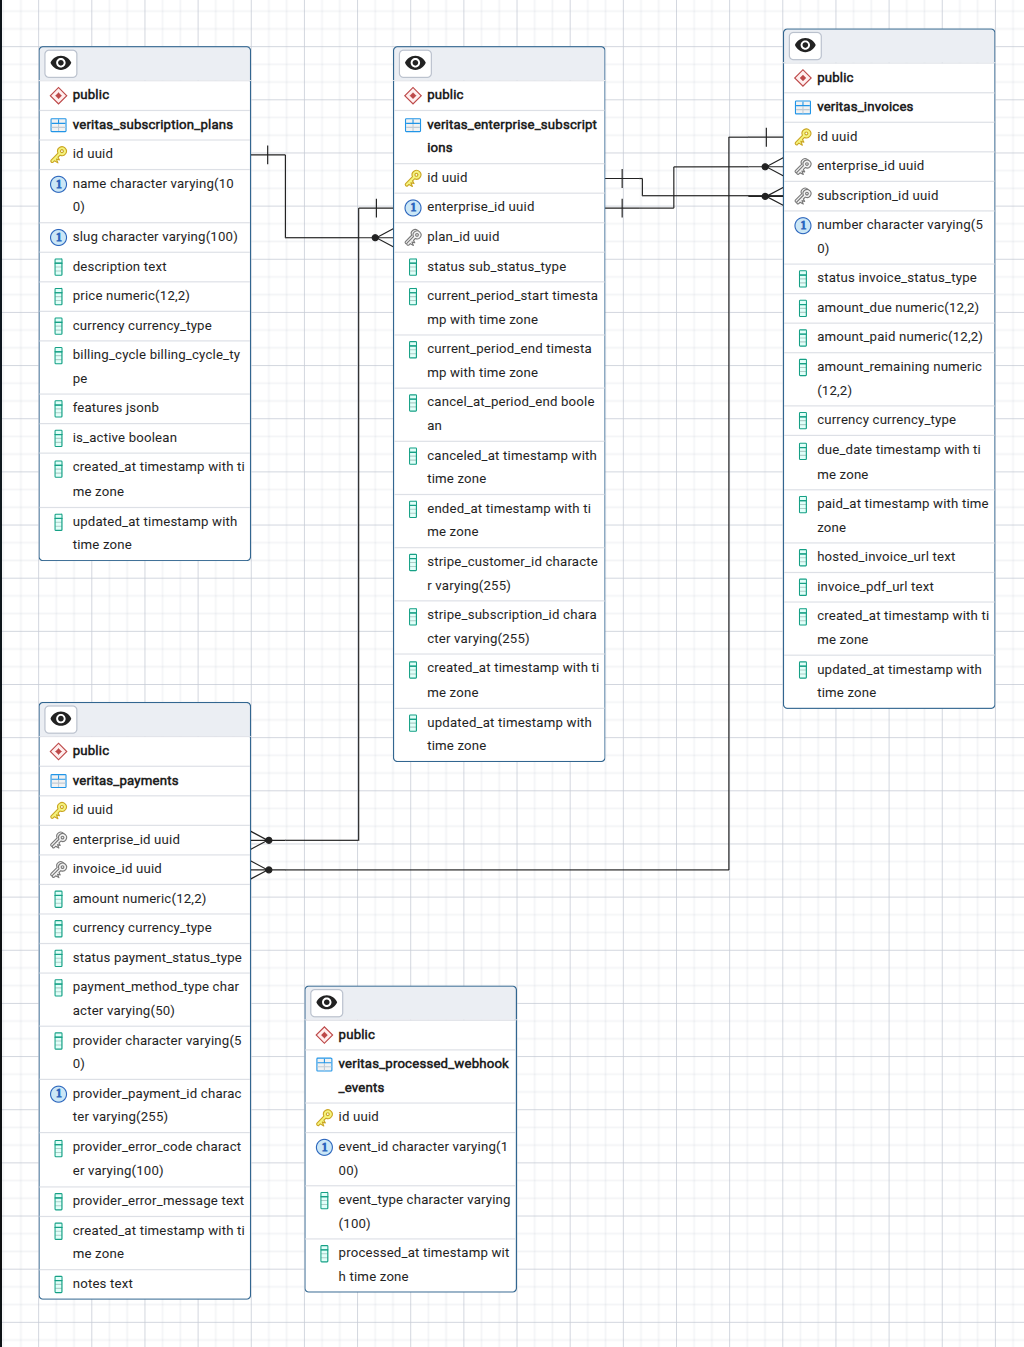
\includegraphics[width=0.95\linewidth,keepaspectratio]{assets/database_erds/payment_svc_db.png}
\caption{Payment Service Database ERD}
\label{fig:erd-payment}
\end{figure}

\begin{figure}[H]
\centering
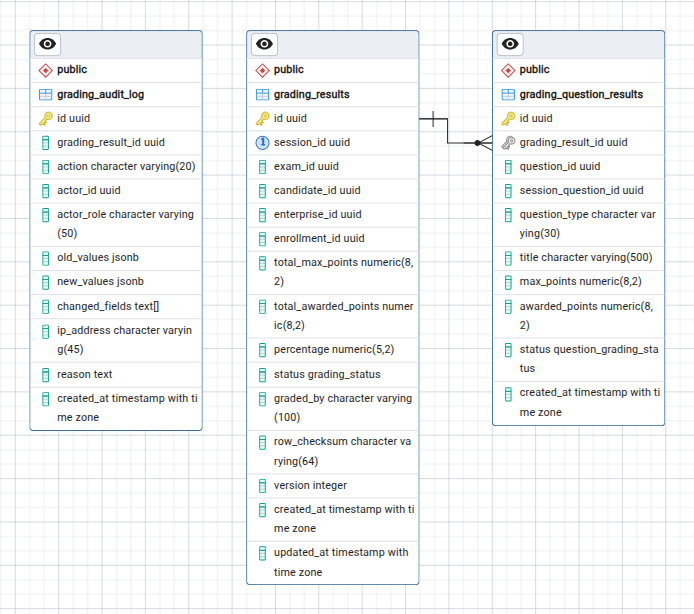
\includegraphics[width=0.95\linewidth,keepaspectratio]{assets/database_erds/grading_svc_db.png}
\caption{Grading Service Database ERD}
\label{fig:erd-grading}
\end{figure}

\begin{figure}[H]
\centering
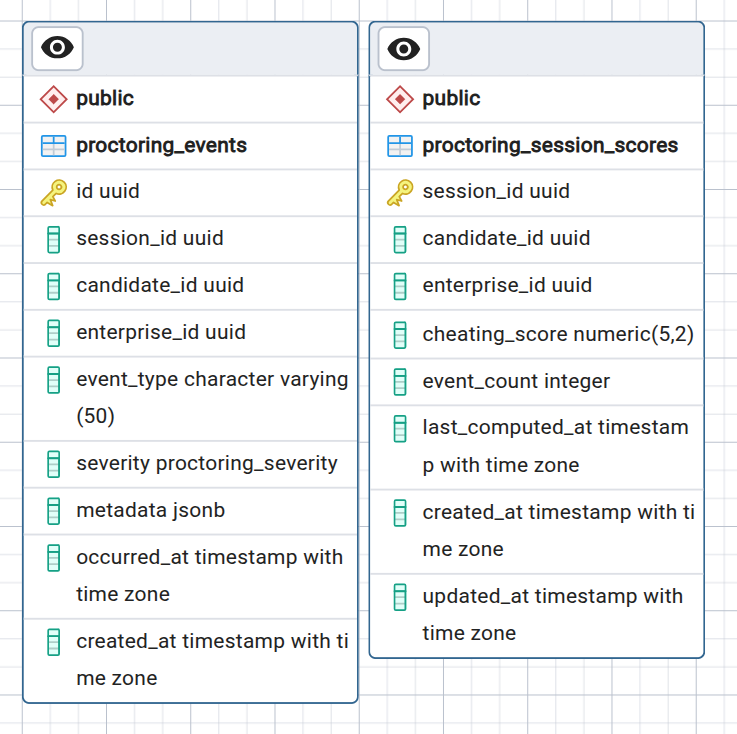
\includegraphics[width=0.95\linewidth,keepaspectratio]{assets/database_erds/proctoring_svc_db.png}
\caption{Proctoring Service Database ERD}
\label{fig:erd-proctoring}
\end{figure}

\paragraph{Data Ownership and Consistency}
Data boundaries are explicitly defined across services to prevent distributed transaction bottlenecks and coupling:
\begin{itemize}
    \item \textbf{Auth Service Schema} (Figure \ref{fig:erd-auth}): Standardizes secure identity credentials, refresh token records, and RBAC bindings.
    \item \textbf{Enterprise Service Schema} (Figure \ref{fig:erd-enterprise}): Manages tenant metadata, staff allocations, and administrative audit logs.
    \item \textbf{Exam Service Schema} (Figure \ref{fig:erd-exam}): Stores isolated question banks, exam templates, and dynamic scheduling criteria.
    \item \textbf{Candidate Service Schema} (Figure \ref{fig:erd-candidate}): Tracks candidate enrollment tokens, active exam sessions status, and raw question-answer states.
    \item \textbf{Payment Service Schema} (Figure \ref{fig:erd-payment}): Records billing metadata, Stripe subscription logs, and transactional invoice events.
    \item \textbf{Grading Service Schema} (Figure \ref{fig:erd-grading}): Persists final computed scores, question-by-question marks, and high-security audit rows backed by row-level cryptographic HMAC checksums.
    \item \textbf{Proctoring Service Schema} (Figure \ref{fig:erd-proctoring}): Houses facial verification logs, eye-tracking events, and aggregated cheating score histories.
\end{itemize}

Cross-service side effects are orchestrated through Kafka event consumers, ensuring eventual consistency. For instance, an enterprise suspension event triggers token revocation in Auth, templates deactivation in Exam, and session termination in Candidate services asynchronously.

\subsubsection{Deployment Diagram}
The system is deployed as containerized services behind the API Gateway. PostgreSQL, Redis, and Kafka run as shared infrastructure containers. Figure \ref{fig:deployment} presents the deployment topology used for local and production environments.

\begin{figure}[H]
\centering
\IfFileExists{assets/system_designs/svg_exports/deployment_diagram_svg-deployment-standalone.pdf}{

\includegraphics[width=1\linewidth,keepaspectratio]{assets/system_designs/svg_exports/deployment_diagram_svg-deployment-standalone.pdf}
}{
\fbox{\parbox{0.9\linewidth}{\centering Placeholder: Deployment Diagram (convert SVG to PDF for final build)}}
}
\caption{Deployment Architecture of the Veritas Platform}
\label{fig:deployment}
\end{figure}

\paragraph{Deployment Notes}
\begin{itemize}
    \item Docker Compose is used for local development, enabling rapid startup of all services.
    \item Kubernetes manifests in the infrastructure directory provide a production-ready deployment model.
    \item Internal service discovery uses DNS and service names within the cluster.
\end{itemize}

\subsubsection{User Interface Design}
This section documents the primary user-facing screens and interfaces developed for the Veritas platform. The UI is built using responsive layouts, adhering to accessibility standards (WCAG 2.1) and incorporating cohesive enterprise branding. Since the final visual design iterations are undergoing final usability checks, high-fidelity placeholder wireframes have been mapped below to outline the operational layout, user flows, and key interactive components.

\begin{figure}[H]
\centering
\fbox{\parbox{0.9\linewidth}{\centering Placeholder: Enterprise Admin Dashboard UI Screenshot}}
\caption{Enterprise Admin Dashboard (Placeholder)}
\label{fig:ui-admin}
\end{figure}

\begin{figure}[H]
\centering
\fbox{\parbox{0.9\linewidth}{\centering Placeholder: Enterprise Staff Exam Management UI Screenshot}}
\caption{Enterprise Staff Exam Management (Placeholder)}
\label{fig:ui-staff}
\end{figure}

\begin{figure}[H]
\centering
\fbox{\parbox{0.9\linewidth}{\centering Placeholder: Candidate Exam Interface UI Screenshot}}
\caption{Candidate Exam Interface (Placeholder)}
\label{fig:ui-candidate}
\end{figure}

\begin{figure}[H]
\centering
\fbox{\parbox{0.9\linewidth}{\centering Placeholder: Proctoring Monitoring View UI Screenshot}}
\caption{Proctoring Monitoring View (Placeholder)}
\label{fig:ui-proctoring}
\end{figure}

\begin{figure}[H]
\centering
\fbox{\parbox{0.9\linewidth}{\centering Placeholder: Grading Results and Override UI Screenshot}}
\caption{Grading Results and Override View (Placeholder)}
\label{fig:ui-grading}
\end{figure}

\paragraph{Enterprise Admin Dashboard}
The dashboard shown in Figure \ref{fig:ui-admin} is the administrative command center for the Enterprise Administrator. It displays real-time aggregated metrics such as active subscription tier status, usage quotas, active exam sessions count, and global candidate success distributions. It provides navigation links to manage administrative staff, customize portal branding, and trigger billing workflows.

\paragraph{Enterprise Staff Exam Management}
The interface illustrated in Figure \ref{fig:ui-staff} is utilized by staff to construct assessment pipelines. Key features include the questions bank manager (supporting drag-and-drop file uploads for multimedia questions), randomized question rule constructors, exam timing windows, enrollment invitations triggers, and manual verification bypass settings.

\paragraph{Candidate Exam Interface}
Figure \ref{fig:ui-candidate} depicts the candidate-facing exam environment. This interface is heavily optimized for low-bandwidth and offline resilience. It renders single-question cards to minimize load time, synchronizes answer states locally using browser local storage, and incorporates persistent sync indicator elements. An integrated proctoring indicator reminds candidates of the active camera and tab-monitoring systems.

\paragraph{Proctoring Monitoring View}
The proctoring screen shown in Figure \ref{fig:ui-proctoring} provides real-time oversight of active assessment sessions. It aggregates deep learning streams from the Proctoring Service, displaying webcam face-matching comparisons, eye-movement tracking metrics, audio anomalies, and browser focus logs. An auto-computed cheating risk score is updated dynamically as events are processed.

\paragraph{Grading Results and Override View}
Illustrated in Figure \ref{fig:ui-grading}, this view presents the final assessment evaluations. It displays side-by-side comparisons of candidate answers alongside AI-generated feedback and awarded scores. It features a secure manual override console where authorized staff can adjust marks; doing so updates the cryptographic row checksum and logs the action in the append-only database audit log with a mandatory justification.

\subsection{Verifying the Requirements in the Design}
This subsection connects the implemented design to the functional and non-functional requirements listed in Chapter 3. The mapping verifies that core requirements are supported by the architecture and deployment decisions.

\subsubsection{Functional Requirements Alignment}
\begin{itemize}
    \item \textbf{Multi-tenant management:} Implemented in Enterprise Service and enforced through tenant-scoped data models and gateway tenant resolution.
    \item \textbf{Secure authentication:} JWT issuance and refresh token management are implemented in Auth Service, with role-based access enforced in the gateway.
    \item \textbf{Exam lifecycle management:} Exam Service provides authoring, scheduling, and publishing; Candidate Service manages sessions and submissions.
    \item \textbf{Proctoring and monitoring:} Proctoring Service handles face verification and behavioral events, with structured proctoring evidence storage.
    \item \textbf{Automated grading:} Grading Service consumes grading triggers and persists results with tamper detection and audit logs.
    \item \textbf{Notifications and billing:} Notification Service consumes Kafka events; Payment Service handles subscription and invoice workflows.
\end{itemize}

\subsubsection{Non-Functional Requirements Alignment}
\begin{itemize}
    \item \textbf{Scalability:} Microservice isolation with asynchronous Kafka workflows supports horizontal scaling.
    \item \textbf{Security and integrity:} JWT-based access control, audit logging, and tamper detection for grades are implemented.
    \item \textbf{Reliability:} Circuit breakers and retry loops for Kafka consumers ensure continued processing under transient failures.
    \item \textbf{Maintainability:} Shared Go modules standardize logging, middleware, and messaging patterns across services.
\end{itemize}

\subsection{Security Model}
This subsection documents the platform's multi-layered security architecture, detailing identity assertion, edge token validation, tenant separation, and the cryptographic and database-level audit systems.

\subsubsection{JWT Access Tokens and Claims}
Veritas enforces a token-based authentication and role-based access control (RBAC) system managed by the \texttt{auth-service}. Upon successful authentication, the service issues cryptographically signed JSON Web Tokens (JWT) using an HMAC-SHA256 signature. The token's payload contains critical authorization claims, which include:
\begin{itemize}
    \item \textbf{Subject (\texttt{sub}):} The globally unique user identifier (UUID) that identifies the authenticated user.
    \item \textbf{Enterprise ID (\texttt{enterpriseId}):} The tenant identifier (UUID) associated with the user's organization, preventing cross-tenant access.
    \item \textbf{Role (\texttt{role}):} The user's role (e.g., \texttt{super\_admin}, \texttt{admin}, \texttt{staff}, \texttt{candidate}), dictating resource access levels.
    \item \textbf{Tier (\texttt{tier}):} The active subscription tier of the enterprise (\texttt{free}, \texttt{pro}, \texttt{enterprise}), which gatekeeps commercial features.
    \item \textbf{Expiration and Issuance:} Standard registered claims (\texttt{exp}, \texttt{iat}) managing token lifecycle and prevention of replay attacks.
\end{itemize}

\subsubsection{Edge Routing and Tenant Scoping at the API Gateway}
To eliminate microservice-level token verification overhead and establish a strict security perimeter, all external HTTP requests pass through the API Gateway, which implements the following pipeline:
\begin{itemize}
    \item \textbf{Authentication Check (\texttt{JWTAuth}):} Validates the signature, expiration, and format of the incoming \texttt{Bearer} token using the shared signing secret.
    \item \textbf{Tenant Resolution (\texttt{TenantResolver}):} Extracts the \texttt{enterpriseId} from the JWT claims and injects it into the routing context.
    \item \textbf{Header Injection (\texttt{InjectUserHeaders}):} Sanitizes and converts JWT claims into standardized HTTP headers:
    \begin{itemize}
        \item \texttt{X-User-ID}: The user's UUID.
        \item \texttt{X-User-Role}: The user's authorized role.
        \item \texttt{X-Enterprise-ID}: The tenant's enterprise UUID.
    \end{itemize}
    \item \textbf{Token Stripping:} The gateway strips the original \texttt{Authorization} header before forwarding the request downstream. Downstream services do not contain JWT parsing logic; they are completely isolated inside the private virtual network and implicitly trust the \texttt{X-User-*} headers injected by the gateway, mitigating signature-spoofing and token propagation overhead.
\end{itemize}

\subsubsection{Audit Mechanisms and Row-Level Integrity}
To maintain absolute auditability and detect malicious manipulation of records, the platform incorporates dual audit strategies:
\begin{itemize}
    \item \textbf{Enterprise Service Audit Trail:} The \texttt{enterprise-service} automatically records administrative operations (e.g., onboarding, role changes, tier modifications, and suspensions) in the \texttt{veritas\_enterprise\_audit\_logs} table. This append-only log captures the actor's UUID, role, action type, specific metadata, and a precise timestamp.
    \item \textbf{Grading Service PL/pgSQL Audit Trigger:} The \texttt{grading-service} implements database-level triggers to enforce data consistency. Any \texttt{INSERT}, \texttt{UPDATE}, or \texttt{DELETE} operation on the \texttt{grading\_results} table automatically fires \linebreak the \texttt{trg\_grading\_results\_audit} trigger. The trigger extracts transaction session variables (such as actor ID, role, IP address, and change reason), compares the before and after states, and logs the change set in a separate \texttt{grading\_audit\_log} table using PostgreSQL \texttt{JSONB} for deep, queryable diffs.
    \item \textbf{Row-Level HMAC Tamper Detection:} To prevent out-of-band updates directly on database tables (e.g., bypassing application logic to alter candidate scores), each record in the \texttt{grading\_results} table features a \texttt{row\_checksum}. \linebreak The \texttt{row\_checksum} is calculated as an HMAC-SHA256 signature using a cryptographically secure \texttt{GRADING\_SECRET\_KEY} over a deterministic string concatenation of the row's immutable scoring parameters:
    \[
    \begin{aligned}
    \text{Message} ={}& \text{session\_id} \mathbin{\Vert} \text{candidate\_id} \mathbin{\Vert} \text{total\_max\_points} \\
    &\mathbin{\Vert} \text{total\_awarded\_points} \mathbin{\Vert} \text{percentage} \mathbin{\Vert} \text{version}
    \end{aligned}
    \]
    Any discrepancy between the calculated hash and the stored \texttt{row\_checksum} during read operations indicates tampering and triggers alert workflows.
    \item \textbf{Optimistic Concurrency Control:} A \texttt{version} column is updated automatically on every legitimate write. Concurrent updates targeting stale record states are automatically aborted.
\end{itemize}

\subsection{Kafka Event Catalogue}
Veritas utilizes an asynchronous message-driven pattern built on Apache Kafka to propagate events across services and process high-latency workloads without direct coupling. Table~\ref{tab:kafka-catalogue} provides the formal event catalog, listing active topics, publishers, consumers, and their structural data contract version.

\begin{landscape}
\begingroup
\small
\setlength{\tabcolsep}{3pt}
\begin{longtable}{|>{\raggedright\arraybackslash}p{3.3cm}|>{\raggedright\arraybackslash}p{2.4cm}|>{\raggedright\arraybackslash}p{2.7cm}|>{\raggedright\arraybackslash}p{5.0cm}|}
\caption{Veritas Platform Kafka Event Catalogue} \label{tab:kafka-catalogue} \\
\hline
\textbf{Topic Name} & \textbf{Publisher} & \textbf{Consumer(s)} & \textbf{Payload Summary and Purpose} \\ \hline
\endfirsthead
\multicolumn{4}{c}%
{{\bfseries Table \thetable\ (continued from previous page)}} \\
\hline
\textbf{Topic Name} & \textbf{Publisher} & \textbf{Consumer(s)} & \textbf{Payload Summary and Purpose} \\ \hline
\endhead
\hline \multicolumn{4}{r}{{Continued on next page}} \\
\endfoot
\hline
\endlastfoot
\path{auth.user.login} & Auth Service & Notification & Emits User ID, IP address, and login timestamp. Used for anomaly detection and login confirmation alerts. \\ \hline
\path{enterprise.enterprise.created} & Enterprise & Notification, Auth & Registers a new tenant onboarding. Initiates baseline schema settings and sends welcome configurations. \\ \hline
\path{enterprise.enterprise.suspended} & Enterprise & Auth, Exam, Candidate & Suspends tenant operations immediately. Revokes JWT session validation and disables ongoing exam templates. \\ \hline
\path{subscription.payment.failed} & Payment & Enterprise, Notification & Stripe-triggered invoice failure. Initiates grace-period counters and notifies the enterprise administrator. \\ \hline
\path{exam.exam.created} & Exam Service & Notification & Broadly updates course/exam configurations. Triggers optional student subscription enrollment calendars. \\ \hline
\path{exam.session.ready_for_grading} & Candidate & Grading Service & Slim trigger v3.0 metadata: session, candidate, and enterprise UUIDs. Initiates async AI evaluation pipeline. \\ \hline
\path{candidate.enrollment.invited} & Candidate & Notification & Outlines candidate invitation details, enrollment token, and branding metadata for dispatching custom invitations. \\ \hline
\path{candidate.exam.submitted} & Candidate & Notification & Emits session UUID and candidate metadata. Triggers an email confirmation containing exam receipts. \\ \hline
\path{proctoring.event.detected} & Proctoring & Reporting, Audit & Logs behavioral proctoring event (e.g. tab-switch, webcam anomaly) with timestamp and event confidence score. \\ \hline
\path{proctoring.cheating_score.updated} & Proctoring & Grading, Reporting & Propagates recomputed session risk metrics and cheating probability scores. Contains a terminal \path{is_final} flag. \\ \hline
\end{longtable}
\endgroup
\end{landscape}

\subsection{Resilience and Failure Handling}
This subsection describes the strategies implemented in Veritas to survive transient hardware, software, or network failures.

\subsubsection{API Gateway Circuit Breaker}
To prevent cascading failures when downstream microservices experience performance degradation or crashes, the API Gateway integrates \texttt{sony/gobreaker} circuit breakers. The circuit breaker operates in three states:
\begin{itemize}
    \item \textbf{Closed State:} Normal operation. All requests are routed downstream. If consecutive failures to a microservice exceed 5 (configured threshold) within a 60-second window, the circuit trips.
    \item \textbf{Open State:} The gateway immediately intercepts and rejects requests targeting the failing microservice, returning an \texttt{HTTP 503 Service Unavailable} error, thereby giving the microservice time to recover.
    \item \textbf{Half-Open State:} After a 30-second cooling-off period, the circuit enters a half-open state, allowing up to 3 test requests through. If all 3 test requests succeed, the breaker returns to the \texttt{Closed} state; if any fail, it trips back to \texttt{Open}.
\end{itemize}

\subsubsection{Slim-Trigger Event Pattern}
Under constrained network conditions (common in regional deployments), transmitting fat messages with large payloads (e.g., full exam templates, candidate responses, and media logs) through Kafka causes network bottlenecks and consumer timeouts. Veritas mitigates this by implementing a \textbf{Slim-Trigger Event Pattern} (v3.0):
\begin{itemize}
    \item When a candidate submits an exam, the \texttt{candidate-service} publishes a minimal event (\texttt{exam.session.ready\_for\_grading}) consisting solely of critical UUID references and versioning tags.
    \item Upon consumption, the \texttt{grading-service} immediately inserts a shell row with \texttt{pending} status into \texttt{grading\_results}. This guarantees that if the candidate or staff calls the status-polling endpoint, they receive a positive acknowledgment (\texttt{pending}) rather than a database \texttt{404 Not Found} error.
    \item The \texttt{grading-service} then issues a lightweight internal synchronous HTTP request to the \texttt{candidate-service} to retrieve the aggregated, target grading payload, evaluating it asynchronously.
\end{itemize}

\subsubsection{Resilient Kafka Consumers}
To ensure robust messaging, all event consumers (e.g., Python \texttt{aiokafka} loops in grading and proctoring services, and Go consumers in auth and notification services) are designed with a recovery pattern:
\begin{itemize}
    \item Consumers run within a persistent asynchronous loop wrapping connection logic in \texttt{try-except} (or Go's \texttt{recover}) blocks.
    \item If connection drops, authentication timeouts, or broker restarts occur, the consumer logs a structured warning and enters a 5-second backoff interval before attempting reconnection, preventing service crash-loops and self-denial of service.
\end{itemize}
